\documentclass{article}
\usepackage[utf8]{inputenc}
\usepackage{amsmath}
\usepackage{amsfonts}
\usepackage{geometry}
\usepackage{listings}
\usepackage{float}
\usepackage{graphicx}
\geometry{a4paper,total={170mm,257mm},left=20mm,top=20mm}

\lstset{language=Java,showstringspaces=false,columns=flexible,basicstyle={\small\ttfamily},
  numbers=none,tabsize=1,breaklines=true,breakatwhitespace=true,prebreak=\space,postbreak=\space}


\title{\texttt{Problem set \# : Solutions}}
\author{\texttt{Unathi Skosana}}
\date{\texttt{\today}}

\begin{document}
  \maketitle

  \begin{lstlisting}[mathescape=true, escapeinside=``, breakautoindent=false]

    `\subsection*{Some problem}`

    Some about minimum information equation....

    `
     \begin{eqnarray*}
         \frac{d}{d\varepsilon} \left[-\int p'(x) \ln\left(\frac{p'(x)}{u(x)}\right)dx -(\lambda_0 - 1)\int p'(x)dx - \beta (\int x^2 p'(x)dx - s^2) \right]_{\varepsilon=0} = 0\\
     \end{eqnarray*}
     `


     Something about the bayesian natural log factor for two hypothesis....

    `
     \begin{figure}[H]
       \centering
       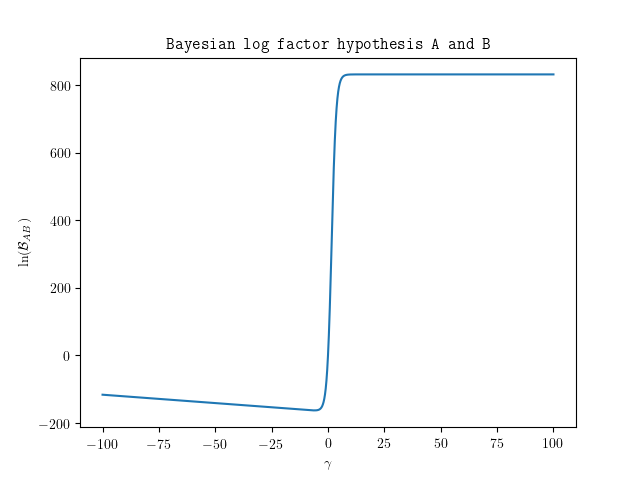
\includegraphics{./resources/Figure_m_20.png}
       \caption{Bayesian Log Factor}
     \end{figure}
    `

    `\subsection*{some other problem}`

    Something about Stirling's approximation and crude approximations for the natural log
    of a factorial, and we compare them via a table.

  \end{lstlisting}

  \begin{table}[h]
    \begin{tabular}{|c|c|c|c|c|c|c|}
    \hline
    $n$ & $f$ & $f_1$ & $\frac{f_1 - f}{f}$ & $g$ & $g_1$ & $\frac{g_1 -g}{g}$ \\ \hline
    5 & 120 & 118.01916 & -0.01650 & 4.78749 & 11.66547 & 1.43665 \\ \hline
    10 & 3628800 & 3598695.61874 & -0.00829 & 15.10441 & 33.72816 & 1.23300 \\ \hline
    15 & 1307674368000 & 1300430722199.468 & -0.00553 & 27.89927 & 59.71520 & 1.14038 \\ \hline
    20 & 2432902008176640000 & 2.42278e+18 & -0.00415 & 42.33561 & 88.25073 & 1.08455 \\
    \hline
    \end{tabular}
  \end{table}


  \begin{lstlisting}[mathescape=true, escapeinside=``, breakautoindent=false]
    It's whatever...
  \end{lstlisting}


\end{document}
